\documentclass[12pt]{amsart}
\usepackage{amsmath}
\usepackage{enumerate}
\usepackage{graphicx}
\graphicspath{{../imgs/}}
\openup 5pt

\author[Blake Farman]{Blake Farman\\University of South Carolina}
\title[Quadratic Worksheet]{Math 111\\Quadratics Worksheet}
\date{November 28, 2017}

\pdfpagewidth 8.5in
\pdfpageheight 11in
\usepackage[margin=1in]{geometry}

\theoremstyle{definition}
\newtheorem{thm}{}
\renewcommand{\qedsymbol}{}

\begin{document}
\maketitle

\vspace{0.2in}
\makebox[\textwidth]{Name:\enspace\hrulefill}
\vspace{0.2in}

Let $f(x) = -3x^2 + 6x + 9$.
Use this function to answer questions Problems~\ref{problem: vertex form}-\ref{problem: graphs}.
\begin{thm}\label{problem: vertex form}
    Write $f(x)$ in vertex form.
\end{thm}
\begin{proof}[Solution]
  We can put $f(x)$ into vertex form by completing the square:
  \begin{eqnarray*}
    f(x) &=& -3x^2 + 6x + 9\\
    &=& -3(x^2 - 2x) + 9\\
    &=& -3(x^2 - 2x + 1 - 1) + 9\\
    &=& -3((x - 1)^2 -1) + 9\\
    &=& -3(x-1)^2 + 3 + 9\\
    &=& -3(x - 1)^2 + 12. 
  \end{eqnarray*}
\end{proof}

\begin{thm}\label{problem: functions and transformations}
  List in order the functions and transformations to get from the graph of $y = x^2$ to the graph of $y = f(x)$.
\end{thm}
\begin{proof}
  We start with the parabola, $y = x^2$.
  \begin{itemize}
  \item
    We obtain $y = (x - 1)^2$ by shifting the parabola right by 1 unit,
  \item
    We obtain $y = 3(x - 1)^2$ by stretching the graph of $y = (x - 1)^2$ by a factor of three,
  \item
    We obtain $y = -3(x - 1)^2$ by reflecting the graph of $y = 3(x - 1)^2$ across the $x$-axis,
  \item
    Finally, we obtain $y = -3(x - 1)^2 + 12 = f(x)$ by shifting the graph of $y = -3(x - 1)^2$ up by 12 units.
  \end{itemize}
\end{proof}

\newpage

\begin{thm}\label{problem: graphs}
  Starting from the graph of $y = x^2$ and ending at the graph of $y = f(x)$, sketch a graph of each of the functions, in order, from your answer to Problem~\ref{problem: functions and transformations}.
  Label the vertex and $y$-intercept on each of your graphs.
\end{thm}
\begin{proof}[Solution]
  In the same order as above, the graphs are as follows:
  \begin{center}
    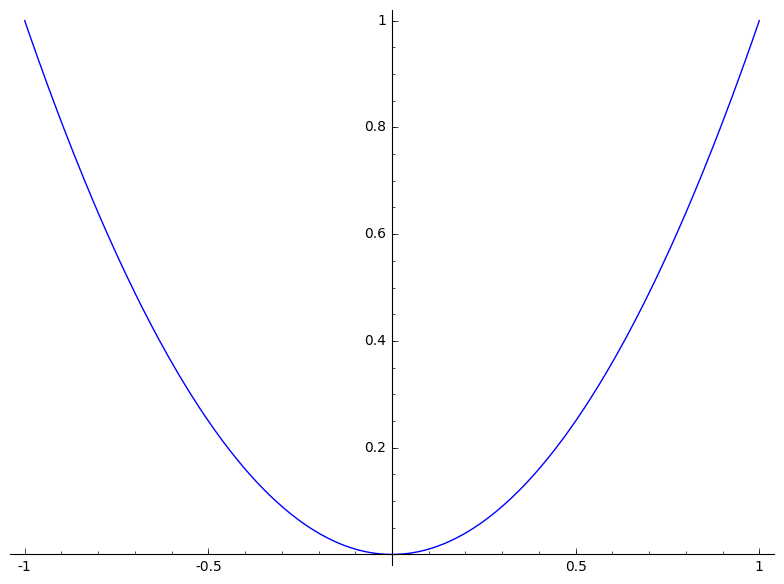
\includegraphics[scale=0.5]{parabola.png}
  \end{center}
  The vertex and $y$-intercept are both $(0,0)$.
  \begin{center}
    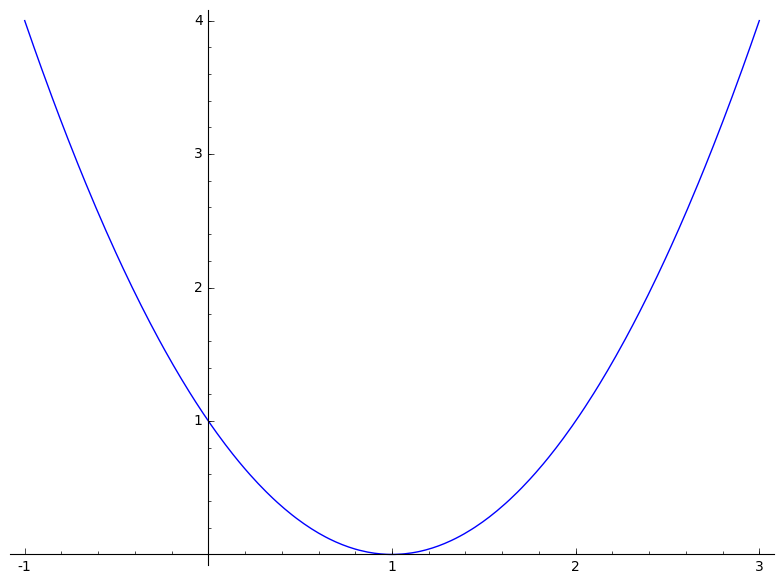
\includegraphics[scale=0.5]{parabolaLeft.png}
  \end{center}
  The vertex is $(1,0)$ and the $y$-intercept is $(0,1)$.
  \begin{center}
    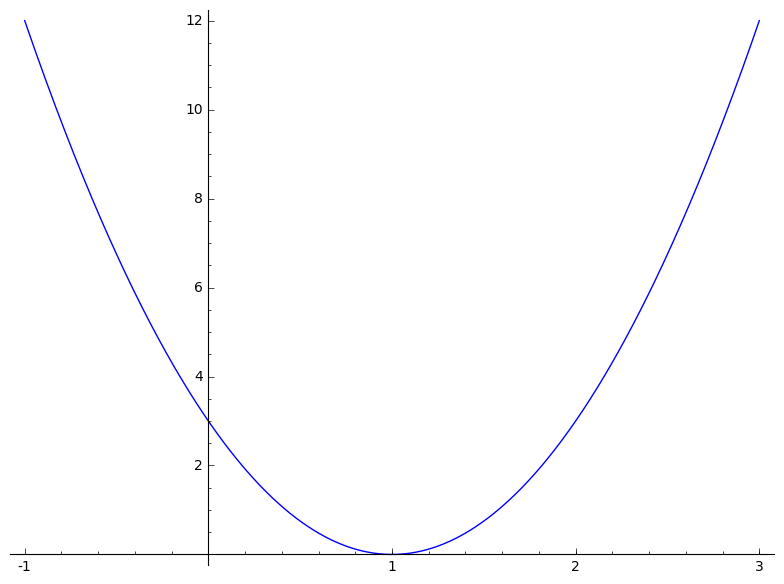
\includegraphics[scale=0.5]{parabolaStretched.png}
  \end{center}
  The vertex is $(1,0)$ and the $y$-intercept is $(0,3)$.
  \begin{center}
    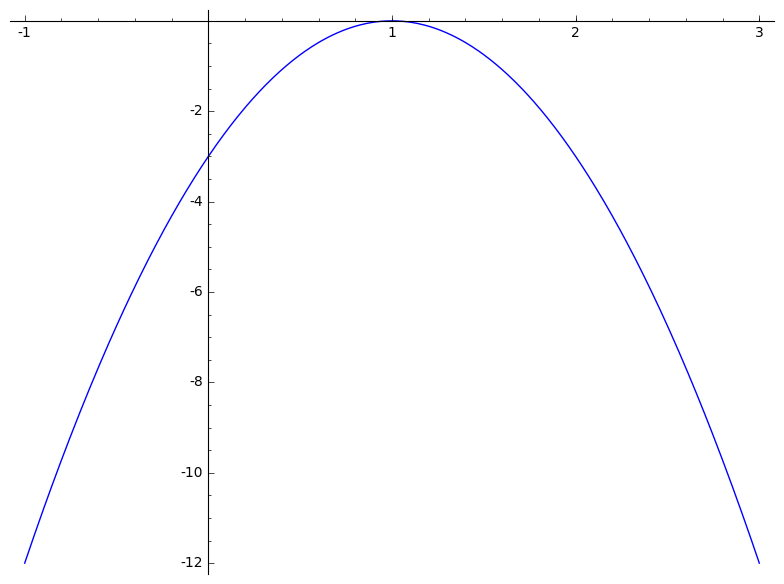
\includegraphics[scale=0.5]{parabolaFlipped.png}
  \end{center}
  The vertex is $(1,0)$ and the $y$-intercept is $(0,-3)$.
  \begin{center}
    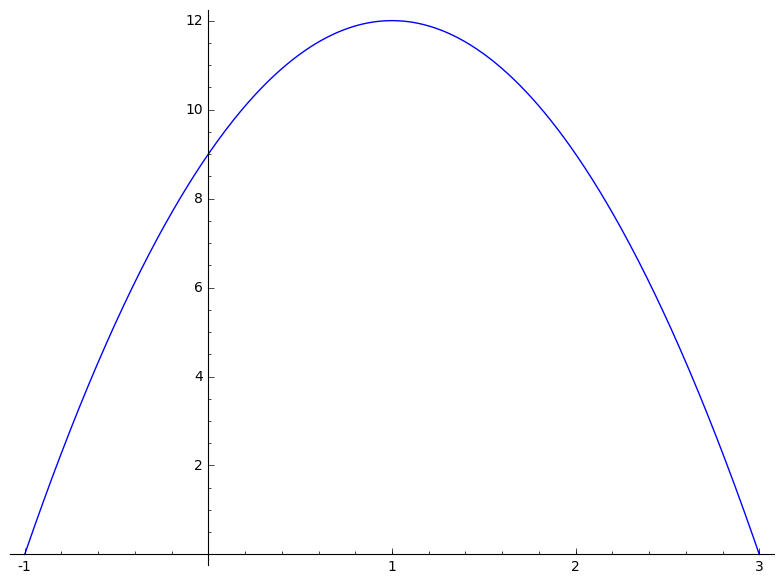
\includegraphics[scale=0.5]{parabolaUp.png}
  \end{center}
  The vertex is $(1,12)$ and the $y$-intercept is $(0,9)$.
\end{proof}

\newpage

\begin{thm}\label{problem: quick and dirty}
  \begin{enumerate}[(a)]
  \item\label{quick and dirty: roots}
    Solve the equation
    $$x^2 - 2x - 8 = 0$$
    for $x$.
    \begin{proof}[Solution]
      Factor
      $$0 = x^2 - 2x - 8 = (x - 4)(x + 2)$$
      to see that either $x = -2$ or $x = 4$.
    \end{proof}
  \item\label{quick and dirty: y-intercept}
    Find the $(x,y)$-coordinates of the $y$-intercept of
    $$y = x^2 - 2x - 8.$$
    \begin{proof}[Solution]
      The coordinates of the $y$-intercept are
      $$(0,0^2 - 2(0) - 8) = (0, 8).$$
    \end{proof}
  \item\label{quick and dirty: vertex}
    Find the $(x,y)$-coordinates of the vertex of
    $$y = x^2 - 2x - 8.$$
    \begin{proof}[Solution]
      The $x$-coordinate of the vertex is
      $$h = \frac{-(-2)}{2(1)} = \frac{2}{2} = 1$$
      and the $y$-coordinate of the vertex is
      $$1^2 - 2(1) - 8 = 1 - 2 - 8 = -9.$$
      Therefore the vertex is at
      $$(1,-9).$$
    \end{proof}
  \end{enumerate}
\end{thm}

\newpage

\begin{thm}\label{problem: graph quick and dirty}
  Use your answers to Problem~\ref{problem: quick and dirty} to sketch a graph of
  $$y = x^2 - 2x - 8 .$$
  Label the $y$-intercept, $x$-intercept(s), and the vertex.
\end{thm}
\begin{proof}[Solution]
  The graph of $y = x^2 - 2x - 8$ is
  \begin{center}
    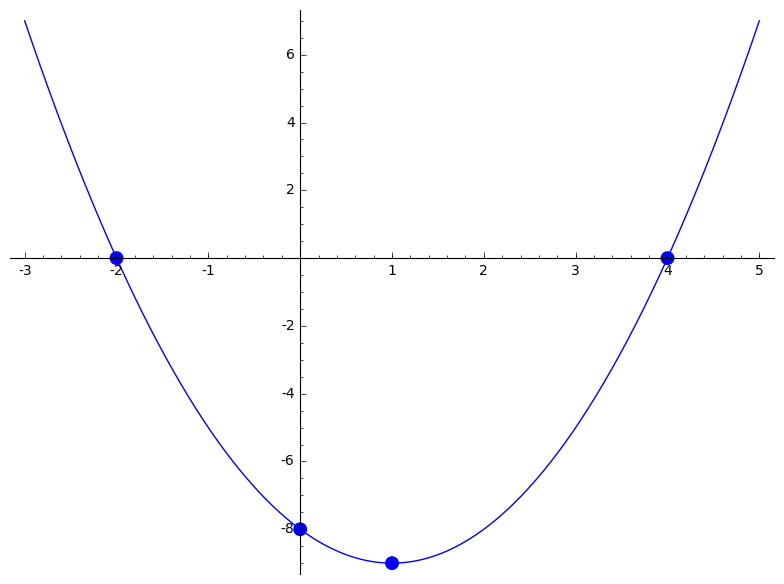
\includegraphics[scale=0.5]{quickanddirty}
  \end{center}
  The coordinates of the marked points, from left to right, are $(-2,0)$, $(0,-8)$, $(1,-9)$, and $(4,0)$.
\end{proof}

\newpage
Bob tosses a ball straight up in the air, then catches it.
When he releases the ball, it leaves his hand at a velocity of 96 feet/sec.
The height of the ball relative to Bob's hand after $t$ seconds can be modeled by the function
$$h(t) = -32t^2 + 96t.$$
Use this model to answer the following Problems.
\begin{thm}\label{problem: kinematics graph}
  Sketch a graph of this function.
  Make sure that your graph is appropriate for this model.
\end{thm}
\begin{proof}[Solution]
  To graph the function $h(t)$, we need the following points
  \begin{itemize}
  \item
    the $y$-intercept: $(0,h(0)) = (0,0)$,
  \item
    the $x$-intercepts:
    Since $0 = h(t) = -16t^2 +96t = -16t^2 + 16(6)(t)= -16t(t - 6)$, they are
    $$(0,0)\ \text{and}\ (3,0),$$
  \item
    the vertex:
    The $x$-coordinate of the vertex is
    $$\frac{-96}{2(-16)} = \frac{3(32)}{32} = 3$$
    so the $y$-coordinate is
    $$h(3) = -16(9) + 96(3) = -16(9 - 18) = -16(-9) = 16(9) = 144.$$
    So the vertex is at
    $$(3,144).$$
  \end{itemize}
  The graph of $h(x)$ is then
  \begin{center}
    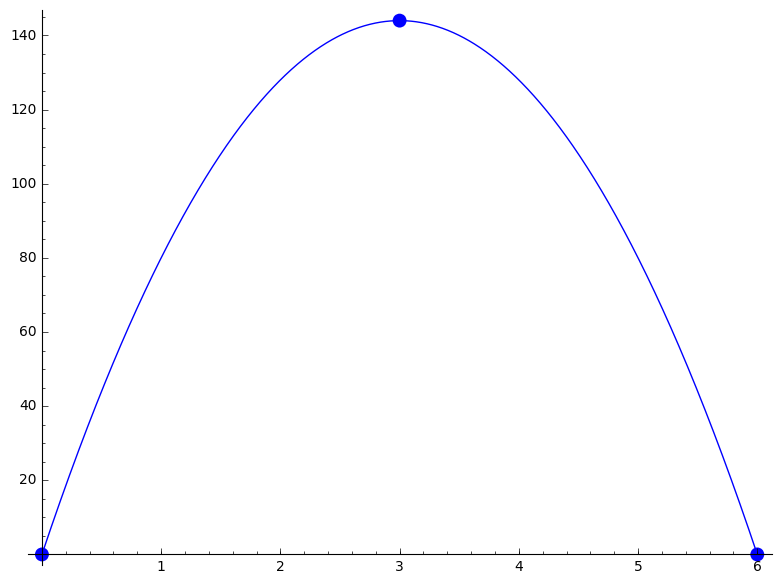
\includegraphics[scale=0.5]{kinematics}
  \end{center}
  Note that this model is only valid for $0 \leq t \leq 6$, since the height of zero at $t = 6$ implies that Bob has caught the ball, and its height is no longer governed by this model.
\end{proof}
\newpage

\begin{thm}\label{problem: maximum}
  Use your answer from the previous problem to answer the following questions.
  \begin{enumerate}[(a)]
  \item
    After how many seconds does the ball reach its maximum height?
    \begin{proof}[Solution]
      Looking at the graph, it's clear that the maximum occurs at the vertex, which is after 3 seconds have elapsed.
    \end{proof}
  \item
    What is the maximum height attained by the ball?
    \begin{proof}[Solution]
      The height is the $y$-coordinate of the vertex, 144 feet.
    \end{proof}
  \item
    After how many seconds does the ball return to Bob's hand?
    \begin{proof}[Solution]
      The ball returns to Bob's hand after 6 seconds; this is the other $x$-intercept.
    \end{proof}
  \end{enumerate}
\end{thm}

\end{document}
